%%%%%%%%%%%%%% 23/02/2020 %%%%%%%%%%%%%%%% 
\subsection*{\textbf{23/02/2020}}

\subsubsection*{Days aims}
\begin{itemize}
    \item Investigate $\Delta \phi$
    \item 
\end{itemize}

\subsubsection*{Day Summary}
\begin{itemize}
    \item Investigated $\Delta \phi$
    \item Applied ptcone30 cut to invariant mass
    \item Plotted etcone20 with ptcone30 cuts
    
    \item Found pT upper cut of:
    \subitem 34 GeV for mumu 
    \subitem 36 GeV for ee 
    
    \item Plotted $\eta$ - ruled out as a cut
    
    \item 
\end{itemize}
%%%%%%%%%%%%% 9:00 %%%%%%%%%%%%%
\subsubsection*{08:30 - Lead BG}
The ATLAS detector can mistake the production of a $l^+ l^-$ pair from 2 seperate decays as pair production from the decay of a single particle, such as a Z boson. 
\\
A possible source of this is from W boson decays:
\begin{align*}
    W^+ \rightarrow l^+ \nu_{l}
    \\
    W^- \rightarrow l^- \Bar{\nu_{l}}
\end{align*}
to be mistaken for $Z \rightarrow ll$.
\\
In the case of $Z \rightarrow ll$, the two leptons would be expected to be produced with the angle between them ($\Delta \phi$) $\approx \pi$ (angle between the azimuthal angle) to conserve momentum.
\\
Counter to this, the  $W^+ \rightarrow l^+ \nu_{l}$ and $W^- \rightarrow l^- \Bar{\nu_{l}}$ can be proceed at any angle, so would expect production to include $\Delta \phi \approx 0$
\\
To investigate this, plot $\Delta \phi$ of ATLAS "2lep" data, the cuts used in Fig.\ref{fig:23-02_09-43} are:
\begin{lstlisting}
lepCut ="(" + "(lep_charge[0] != lep_charge[1]) && (lep_type[0]==13 && lep_type[1]==13) && lep_n==2 && (inv_mass_Zll > 60e3)" + ")"
    
t.SetAlias("inv_mass_Zll","sqrt(2*lep_pt[0]*lep_pt[1]*(cosh(lep_eta[0]-lep_eta[1])-cos(lep_phi[0]-lep_phi[1])))")

t.Draw("abs(lep_phi[0] - lep_phi[1]) >> h_lep_delta_phi(100,0,6.3)", weighting + "*" + lepCut)
\end{lstlisting}

Fig.\ref{fig:23-02_09-43} shows that there is a small peak at loer angles.  This can be produced from. two main processes:
\begin{itemize}
    \item Momentum conservation to compensate for jets
    \item incorrect classification for two W+ and W- decays.
\end{itemize}

\begin{figure}[h!]
    \centering
    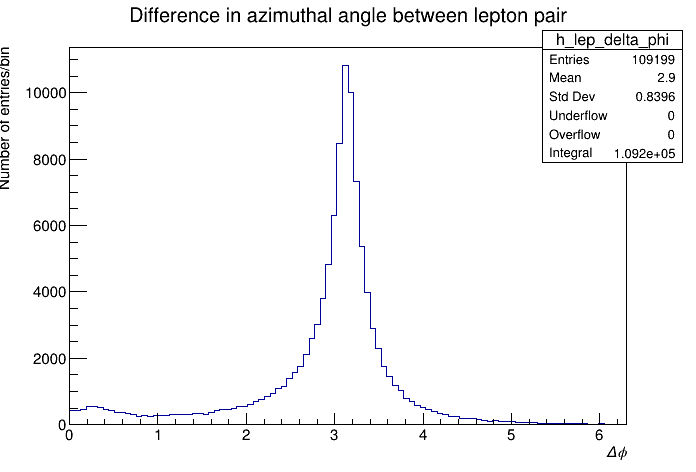
\includegraphics[width=0.85\linewidth]{plots/23-02-2021/2lep_delta-phi_0-7_23-02_09-43.png}
    \caption{The difference of the azimuthal angle of the lepton pair for the 2lep ATLAS data.  The main peak at approx $\pi$ is as expected}\label{fig:23-02_09-43}
\end{figure}

%%%%%%%%%%%%% 9:48 %%%%%%%%%%%%%
\subsubsection*{09:48 - Lead DG}
Apply ptcone20 cut on invariant mass plots.
\\
Since there is no distinction between events in the range 0-1 GeV, cut events above 1 GeV.
\\
Since variables/quantities are correlated (can be effected by the same physical process), plot the etcone20 stack plot.   See Fig.\ref{}

%%%%%%%%%%%%% 14:07 %%%%%%%%%%%%%
\subsubsection*{14:07 - Lead BG}
Plot pT log to test for potential cuts.

Test other kinematic variables to look for potential cuts

Upper bound cut of 320GeV for total lepton pair pT.  See Fig.{}

%%%%%%%%%%%%% 15:24 %%%%%%%%%%%%%
\subsubsection*{15:24 - Lead DG - Plot $\eta$}
Plot eta in search of potential cuts. 
\\
Cuts used for Fig.\ref{fig:15-24_23-02-21}:
\begin{lstlisting}
lepCut ="(" + "(lep_charge[0] != lep_charge[1]) && (lep_type[0]==lep_type[1]) && lep_n==2" + ")"
    
t.Draw("abs(lep_eta[0]) >> h_lep_eta(100,0,3)", weighting + "*" + lepCut)
\end{lstlisting}
\begin{figure}[h!]
    \centering
	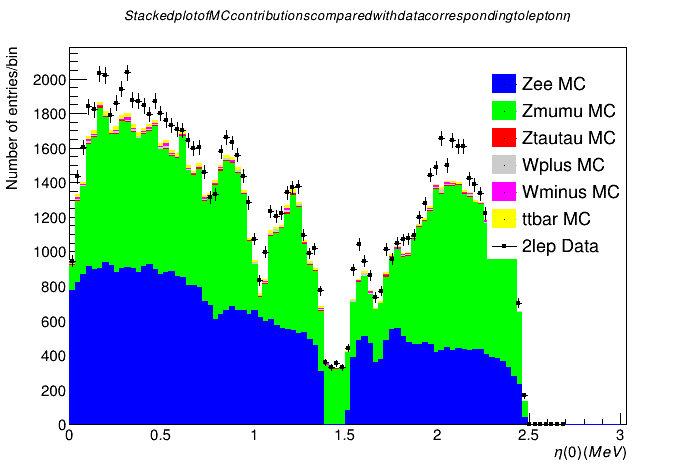
\includegraphics[width=0.85\linewidth]{plots/23-02-2021/All-stack-fast_eta_0-3_.png}
	\caption{Stack plot for the absolute value of $eta$ for lepton [0] to include signal and and background 2lep and MC.  Cuts: lepton pair of same flavour/type and opposite charge. }\label{fig:15-24_23-02-21}
\end{figure}


%%%%%%%%%%%%% 15:31 %%%%%%%%%%%%%
\subsubsection*{15:31}
Plot the stack plot of delta phi in search of possible cuts.
\\
First apply only minimal cuts (no lower from invariant mass and upper ):
\begin{lstlisting}
lepCut ="(" + "(lep_charge[0] != lep_charge[1]) && (lep_type[0]==13 && lep_type[1]==13) && lep_n==2 && (inv_mass_Zll > 60e3)" + ")"
    
t.SetAlias("inv_mass_Zll","sqrt(2*lep_pt[0]*lep_pt[1]*(cosh(lep_eta[0]-lep_eta[1])-cos(lep_phi[0]-lep_phi[1])))")

t.Draw("abs(lep_phi[0] - lep_phi[1]) >> h_lep_delta_phi(100,0,6.3)", weighting + "*" + lepCut)
\end{lstlisting}
\begin{figure}[h!]
    \centering
	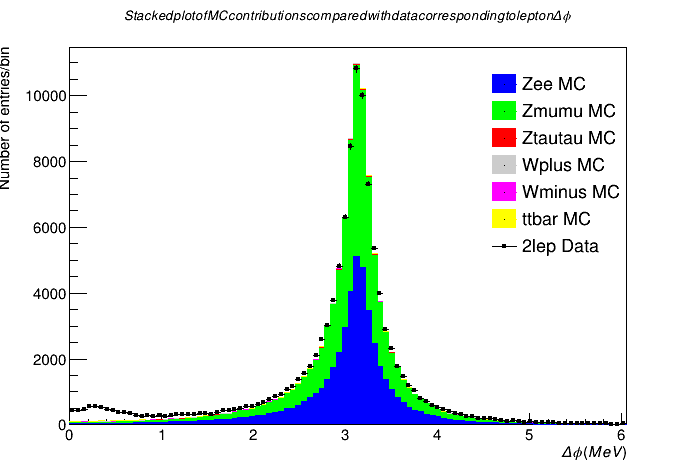
\includegraphics[width=0.85\linewidth]{plots/23-02-2021/All-stack-fast_delta-phi_minimal-cuts_0-6_23-02-21_15-30.png}
	\caption{Stack plot of delta phi with only minimal cuts to select for events with 2 leptons of same type with opposite charge.  There is an inconstancy between MC and ATLAS data (\textbf{NOT MeV - should be rad})}\label{fig:All-stack-fast_delta-phi_minimal-cuts_0-6_23-02-21_15-30}
\end{figure}
From Fig.\ref{fig:All-stack-fast_delta-phi_minimal-cuts_0-6_23-02-21_15-30}:
- Inconstancy between MC and ATLAS data around 0-1 rad.

Now add upper from total transverse momentum and lower from invariant mass.
\begin{figure}[h!]
    \centering
	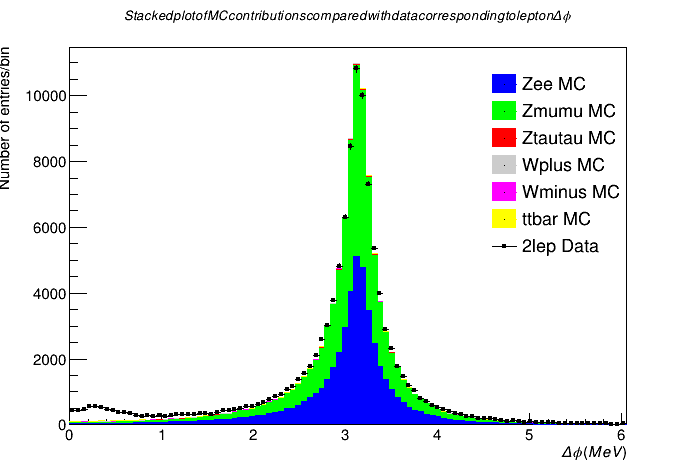
\includegraphics[width=0.85\linewidth]{plots/23-02-2021/All-stack-fast_delta-phi_minimal-cuts_0-6_23-02-21_15-30.png}
	\caption{Stack plot of delta phi with only minimal cuts to select for events with 2 leptons of same type with opposite charge.  There is an inconsitancy between MC and ATLAS for $\Delta \phi < 1 rad$ (\textbf{NOT MeV - should be rad})}\label{fig:All-stack-fast_delta-phi_minimal-cuts_0-6_23-02-21_15-30}
\end{figure}
From Fig.\ref{}:
-> Good MC fit to ATLAS data - no more "bump" between 0-1 rad

Question: Is it better to make cuts based on individual particles or total/mean.
 
 %%%%%%%%%%%%% 15:54 %%%%%%%%%%%%%
\subsubsection*{15:54 - Lead BG}
Start to calculate the cross section of $pp \rightarrow Z \rightarrow ee$ with the new cuts (lower and upper bounds on variables).
\\
Cuts being used:
\begin{lstlisting}
lepCut ="(" + "(lep_charge[0] != lep_charge[1]) && (lep_type[0]==lep_type[1]) && lep_n==2 && (inv_mass_Zll > 60e3) && (lep_pt[0]+lep_pt[1]) < 320e3 " + ")"
\end{lstlisting}

%%%%%%%%%%%%% 17:00 %%%%%%%%%%%%%
\subsubsection*{17:00 - Logout}